% --------------------------------------------------------------------
% This is a simple Beamer document that uses beamerthemesigma.sty
% Reading the comments should help you create a presentation even if
% you've never used Beamer before.
% --------------------------------------------------------------------
% Set our document class to Beamer
\documentclass[aspectratio=169, 11pt, handout]{beamer}

% Some packages for nice font encodings in the final PDF
%\usepackage[utf8]{inputenc}
\usepackage[T1]{fontenc}

% Emoji?
\usepackage{emoji}

% Good tables
\usepackage{booktabs}
\usepackage{tabularx}
\usepackage{colortbl}

\usepackage{mathtools}
\newcommand\nindent{.5pt}
\newcommand\noverline[1]{%
  \kern\nindent\overline{\kern-\nindent#1\kern-\nindent}\kern\nindent}
\newcommand\midoverline[1]{%
  \sbox0{$#1$}%
  \bgroup\ooalign{$#1$\cr$\noverline{\rule{.5\wd0}{0pt}\vphantom{#1}}%
  \noverline{\rule{.5\wd0}{0pt}\vphantom{#1}}$}\egroup
}

% To insert images
\usepackage{graphicx}
\usepackage{multicol}
% Useful packages from the AMS
\usepackage{amsmath,amssymb,amsthm}

% Package for code highlighting
\usepackage{minted}
\setminted{linenos=true, breaklines=true, breakanywhere=true, style=default}
\usemintedstyle{monokai}

% Set a title
\title{Let's Build a Computer!}

% The subtitle is generally where I'd expect you to put the week
% number, thus:
\subtitle{Week 3}

% Whoever worked on the presentation:
\author{Aditya ({\color{sigma@mainblue}\textsf{@nebu}})}

% A date, if you'd like.
\date{}

% An institute name, if you're so inclined
% \institute{University of Illinois Urbana-Champaign}

% Use the SIGma theme for this Beamer presentation
\usetheme{sigma}
% --------------------------------------------------------------------
% Begin document
\begin{document}

% Beamer calls each slide a "frame", defined within the environment:
% \begin{frame}
%   <frame content here>
% \end{frame}

% This frame is just the title.
\begin{frame}
\titlepage
\end{frame}

% A frame with the table of contents.
% This frame's title is "Outline".
\begin{frame}{Outline}
  \tableofcontents
\end{frame}

\begin{frame}{Why Are We Doing This?}
  % Let's put some real content in this frame:
  \pause
  \begin{itemize}
    \item Understanding automata theory means understanding, in part,
        what the things in this figure mean:
        \begin{center}
        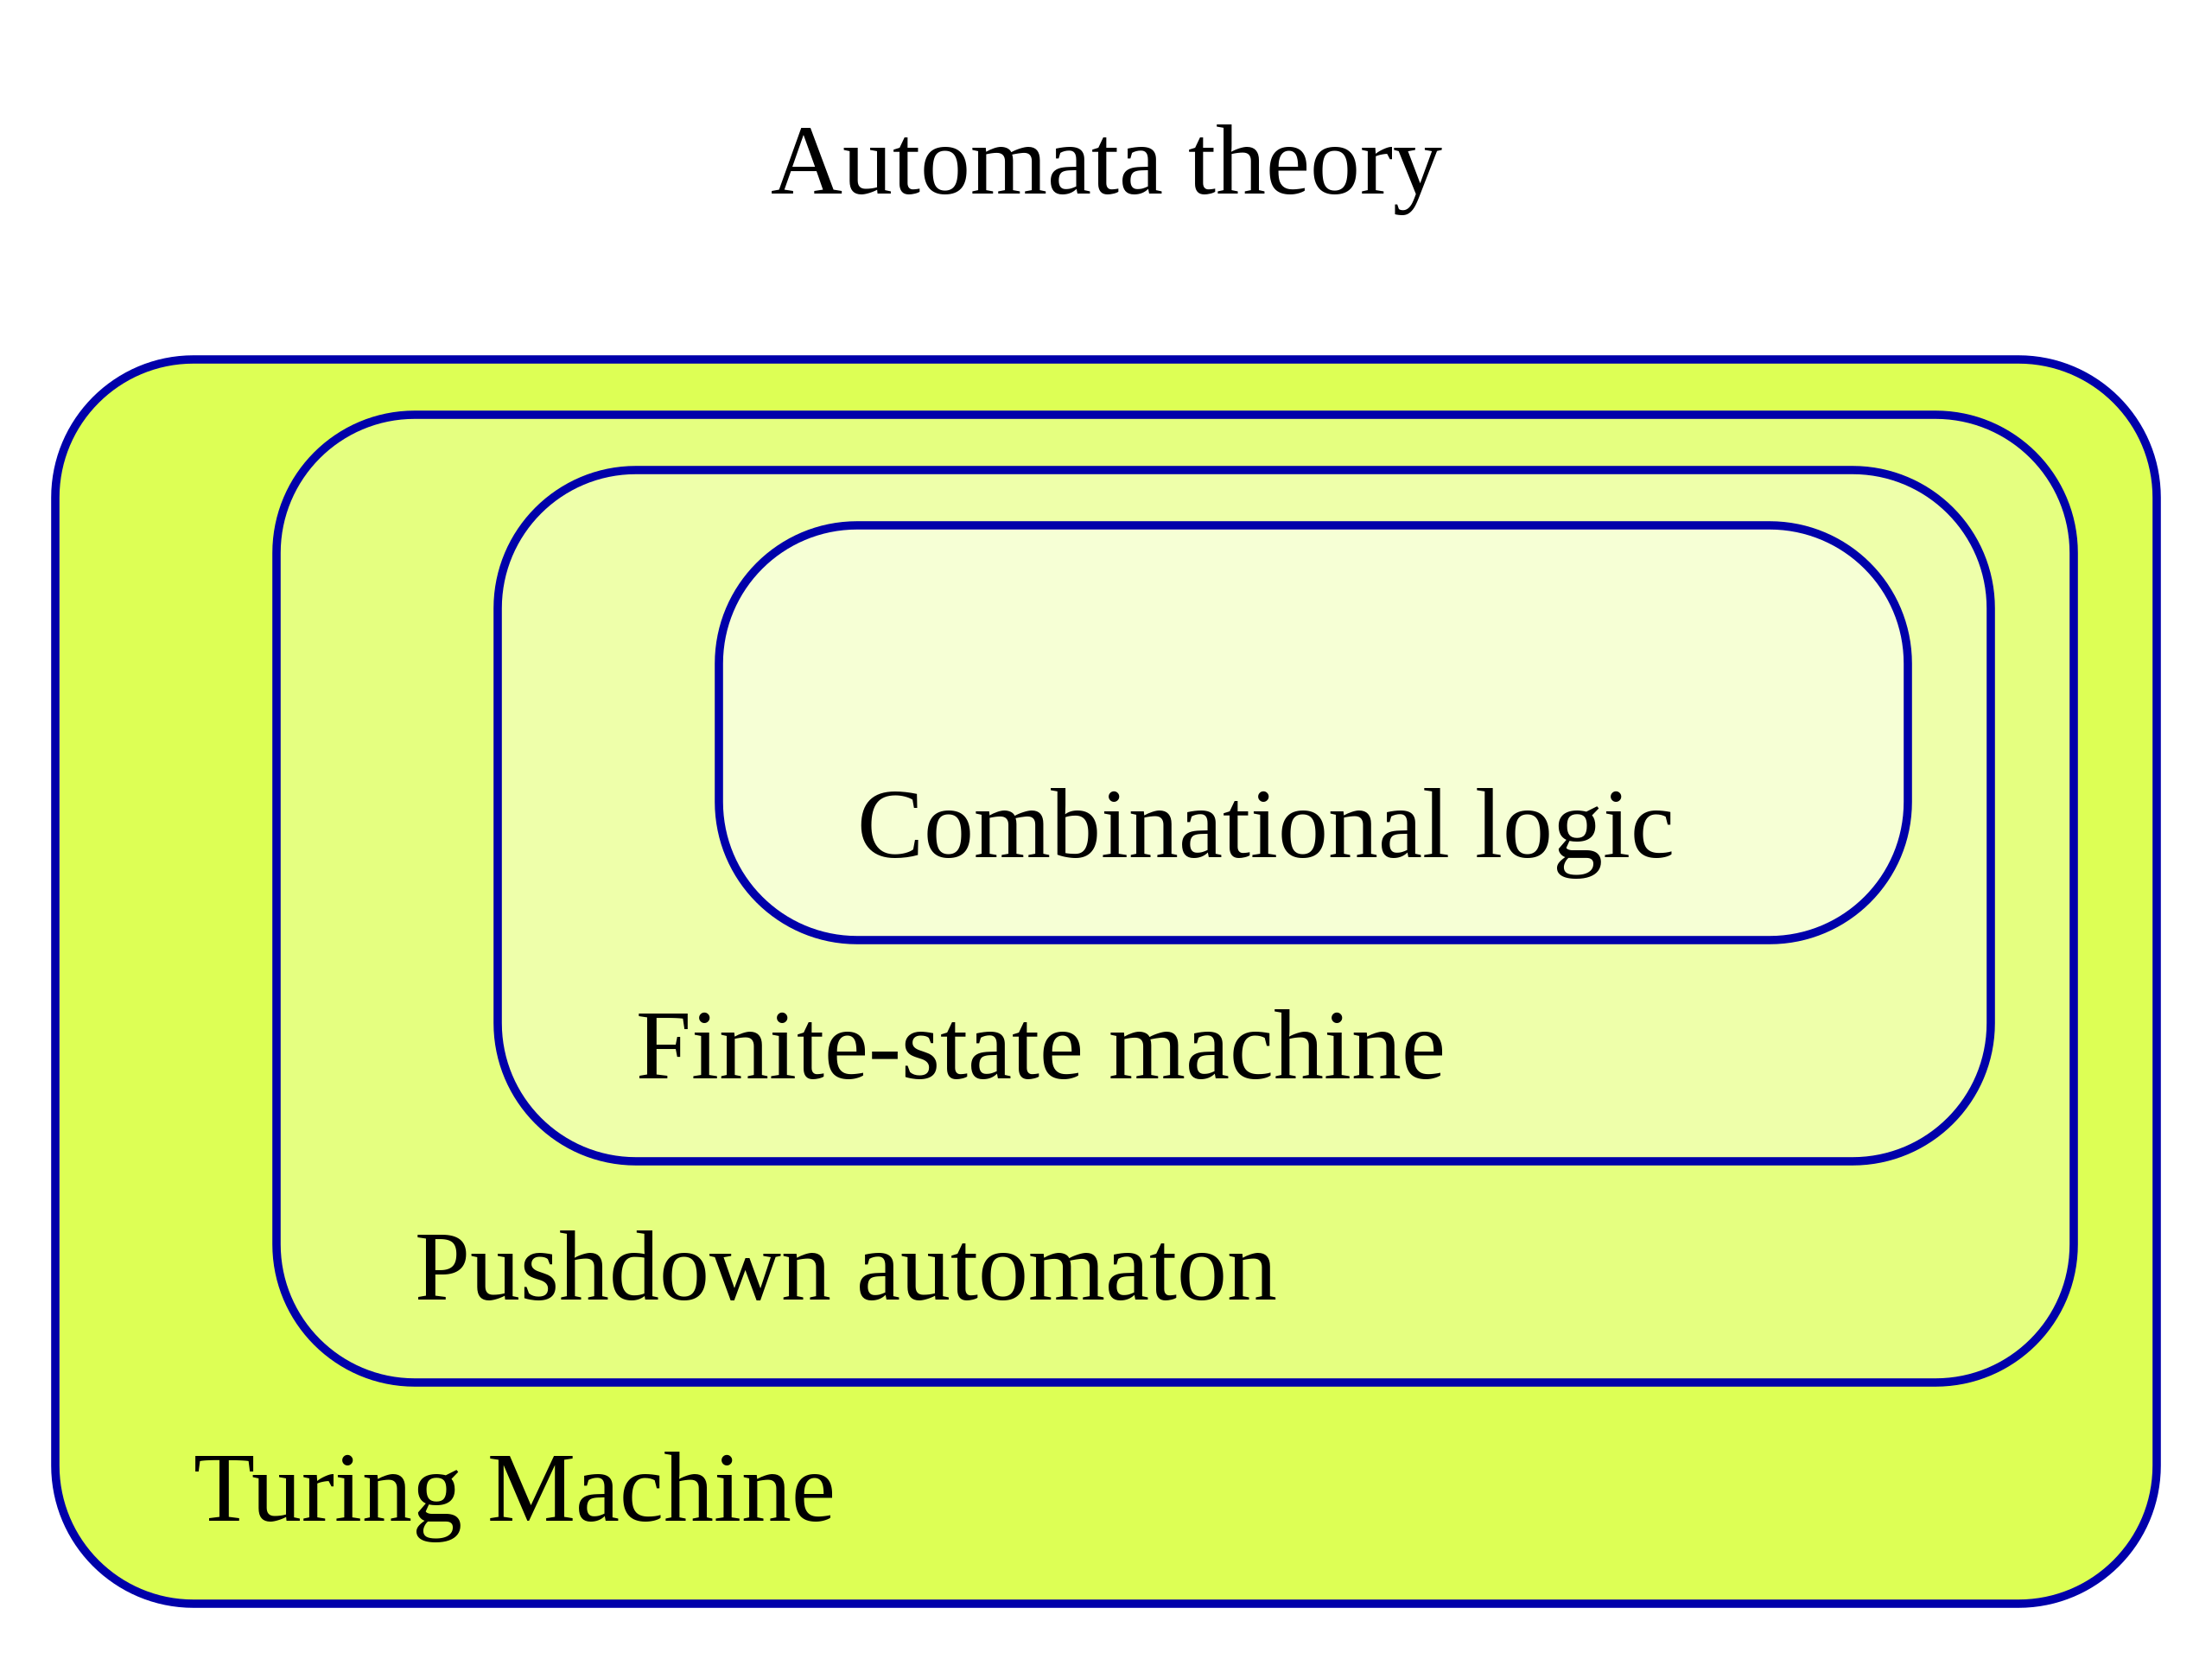
\includegraphics[width=0.6\textwidth]{2560px-Automata_theory.png}
        \end{center}
  \end{itemize}
\end{frame}

\begin{frame}{Why Are We Doing This?}

  \begin{itemize}
    \item Understanding automata theory means understanding, in part,
        what the things in the figure on the previous slide mean. 
        \item Teaches an application of what we're learning.\pause
        \item Shows how general and useful the ideas we're covering are. ({\color{sigma@mainblue}\textsf{@Hassam}} compilers soon? \emoji{eyes})\pause
        \item Is very rewarding since computers are everywhere.
  \end{itemize}
\end{frame}
% Start a section: *sections* (subsections, etc.) are what show up in the TOC.
\section{Combinational Logic}
% Section pages can be printed thus:
\frame{\sectionpage}
% There's a way to automate this, see:
% https://tex.stackexchange.com/questions/178800/creating-sections-each-with-title-pages-in-beamers-slides/178803


% Another frame:
\begin{frame}
  % Alternate syntax for frame titles
  \frametitle{NOT Gate}
\begin{columns}
\begin{column}{0.5\textwidth}
\centering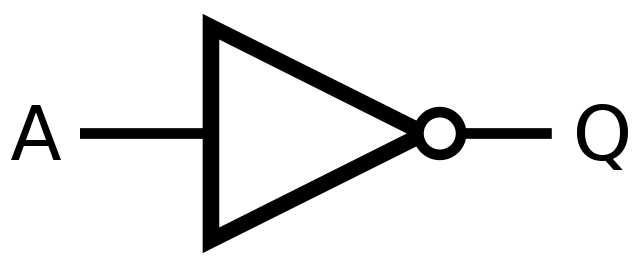
\includegraphics[width=0.5\textwidth]{640px-NOT_ANSI_Labelled.png}
\end{column}
\begin{column}{0.5\textwidth}

\begin{center}
\begin{tabular}{c|c}
\toprule
$A$ & $Q = \overline{A}$\\
\midrule
0 & 1\\
1 & 0\\
\bottomrule
\end{tabular}
\end{center}
\pause
\end{column}
\end{columns}
\end{frame}

% Another frame:
\begin{frame}
  % Alternate syntax for frame titles
  \frametitle{AND Gate}
\begin{columns}
\begin{column}{0.5\textwidth}
\centering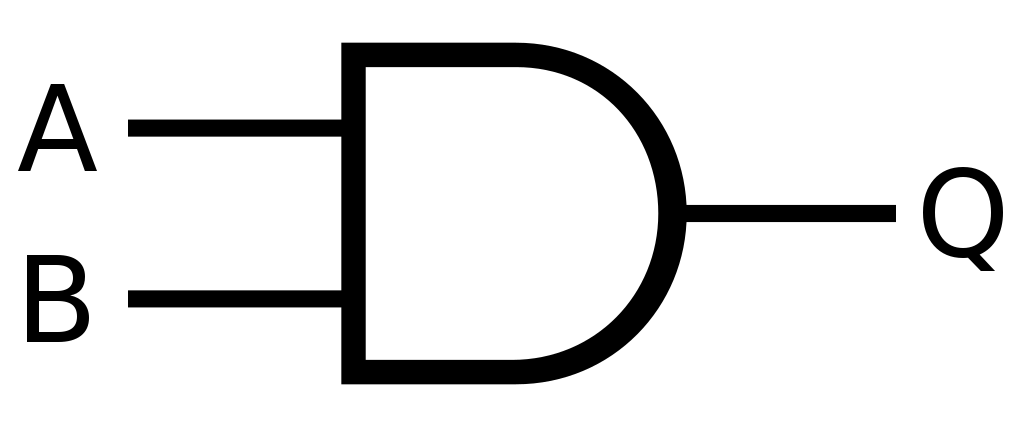
\includegraphics[width=0.5\textwidth]{1024px-AND_ANSI_Labelled.png}
\end{column}
\begin{column}{0.5\textwidth}

\pause
\begin{center}
\begin{tabular}{cc|c}
\toprule
$A$ & $B$ & $Q=AB$\\
\midrule
0 & 0 & 0\\
0 & 1 & 0\\
1 & 0 & 0\\
1 & 1 & 1\\
\bottomrule
\end{tabular}
\end{center}

\end{column}
\end{columns}
\end{frame}

% Another frame:
\begin{frame}
  % Alternate syntax for frame titles
  \frametitle{OR Gate}
\begin{columns}
\begin{column}{0.5\textwidth}
\centering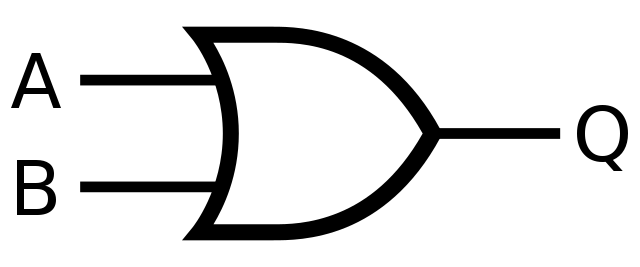
\includegraphics[width=0.5\textwidth]{640px-OR_ANSI_Labelled.png}
\end{column}
\begin{column}{0.5\textwidth}

\pause
\begin{center}
\begin{tabular}{cc|c}
\toprule
$A$ & $B$ & $Q=A+B$\\
\midrule
0 & 0 & 0\\
0 & 1 & 1\\
1 & 0 & 1\\
1 & 1 & 1\\
\bottomrule
\end{tabular}
\end{center}

\end{column}
\end{columns}
\end{frame}



\begin{frame}{That's It!*}
   \pause
   
  \begin{itemize}
      \item AND, OR, and NOT are functionally complete.\pause%\footnote{In fact, there's an isomorphism between Boolean logic and the algebra of sets, which is also functionally complete.}
      \item This means we can turn any ``Boolean'' function into one that's made up of \textbf{only} ANDs, ORs, and NOTs.
  \end{itemize}
\end{frame}

\begin{frame}{Constructive Proof}
\begin{columns}
\begin{column}{0.5\textwidth}
    \begin{center}
\begin{tabular}{ccc|c}
\toprule
A & B & C & Q\\
\midrule
0 & 0 & 0 & 0\\
0 & 0 & 1 & 1\\
0 & 1 & 0 & 0\\
0 & 1 & 1 & 1\\
1 & 0 & 0 & 1\\
1 & 0 & 1 & 0\\
1 & 1 & 0 & 0\\
1 & 1 & 1 & 1\\
\bottomrule
\end{tabular}
\end{center}
\end{column}
\begin{column}{0.5\textwidth}
\end{column}
\end{columns}
\end{frame}

\begin{frame}{Constructive Proof}
\begin{columns}
\begin{column}{0.5\textwidth}
    \begin{center}
\begin{tabular}{ccc|c}
\toprule
A & B & C & Q\\
\midrule
0 & 0 & 0 & 0\\
\rowcolor{yellow}0 & 0 & 1 & 1\\
0 & 1 & 0 & 0\\
 \rowcolor{yellow}0 & 1 & 1 & 1\\
 \rowcolor{yellow}1 & 0 & 0 & 1\\
1 & 0 & 1 & 0\\
1 & 1 & 0 & 0\\
 \rowcolor{yellow}1 & 1 & 1 & 1\\
\bottomrule
\end{tabular}
\end{center}
\end{column}\pause
\begin{column}{0.5\textwidth}
$$Q = \noverline{A}\noverline{B}C \pause+ \noverline{A}BC \pause+ A\noverline{B}\noverline{C} \pause+ ABC$$

\pause

This works because we ``look for'' all combinations of A, B, and C that'll make Q high. If any of those combinations are high, Q is high.

\end{column}
\end{columns}
\end{frame}


\begin{frame}{}
      \begin{center}
    {\color{sigma@mainblue} \bfseries\LARGE Questions?}
  \end{center}
\end{frame}


\begin{frame}{Questions!}
    Write F as an expression of A, B, and S.
    
\begin{center}
\begin{tabular}{ccc|c}
\toprule
S & A & B & F\\
\midrule
0 & 0 & 0 & 0\\
0 & 0 & 1 & 0\\
0 & 1 & 0 & 1\\
0 & 1 & 1 & 1\\
1 & 0 & 0 & 0\\
1 & 0 & 1 & 1\\
1 & 1 & 0 & 0\\
1 & 1 & 1 & 1\\
\bottomrule
\end{tabular}
\end{center}
\end{frame}

\begin{frame}{Solution}
    
\begin{columns}
\begin{column}{0.5\textwidth}
    $$F = \overline{S}A + SB$$
    \end{column}
    
\pause
\begin{column}{0.5\textwidth}
\begin{center}
    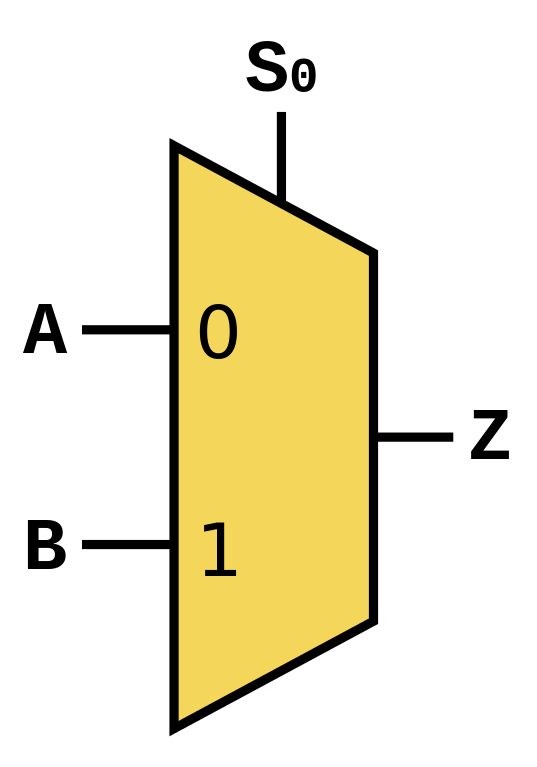
\includegraphics[width=0.5\textwidth]{537px-Multiplexer_2-to-1.png}
\end{center}
    \end{column}
    \end{columns}
\end{frame}

\begin{frame}{Takeaways Before We Move On}
    \begin{itemize}
        \item We can now map any input bits to output bits.\pause
        \item You can build any Boolean function using only AND, OR, and NOT.\pause
        \item Using this knowledge, you can build adders, multipliers, decoders, priority MUXes...whatever you want really.
    \end{itemize}
\end{frame}

\section{Feedback and FSMs}
\frame{\sectionpage}

\begin{frame}{A Fly in the Soup}
    \begin{itemize}
        \item When I said you could build anything you wanted, what did I miss?\pause
        \item \textbf{Storage.}\pause
        \item Any ideas?
    \end{itemize}
\end{frame}


\begin{frame}{Consider This: No Longer Combinational}
    \begin{center}
        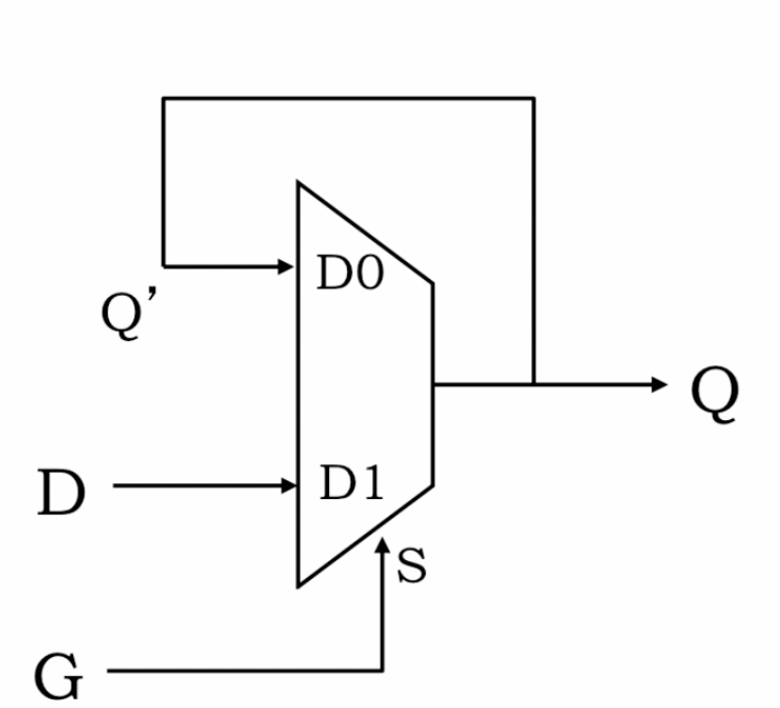
\includegraphics[width=0.5\textwidth]{Screen Shot 2022-09-25 at 00.14.12.png}
    \end{center}
\end{frame}

\begin{frame}{That's a Latch}
    It's rarely used as a memory element --- can you guess why?\\\pause
    
    \emph{Latches are level triggered.}
    
\end{frame}

\begin{frame}{To Explain This, Let's Talk About Cars}
\pause

\begin{center}
    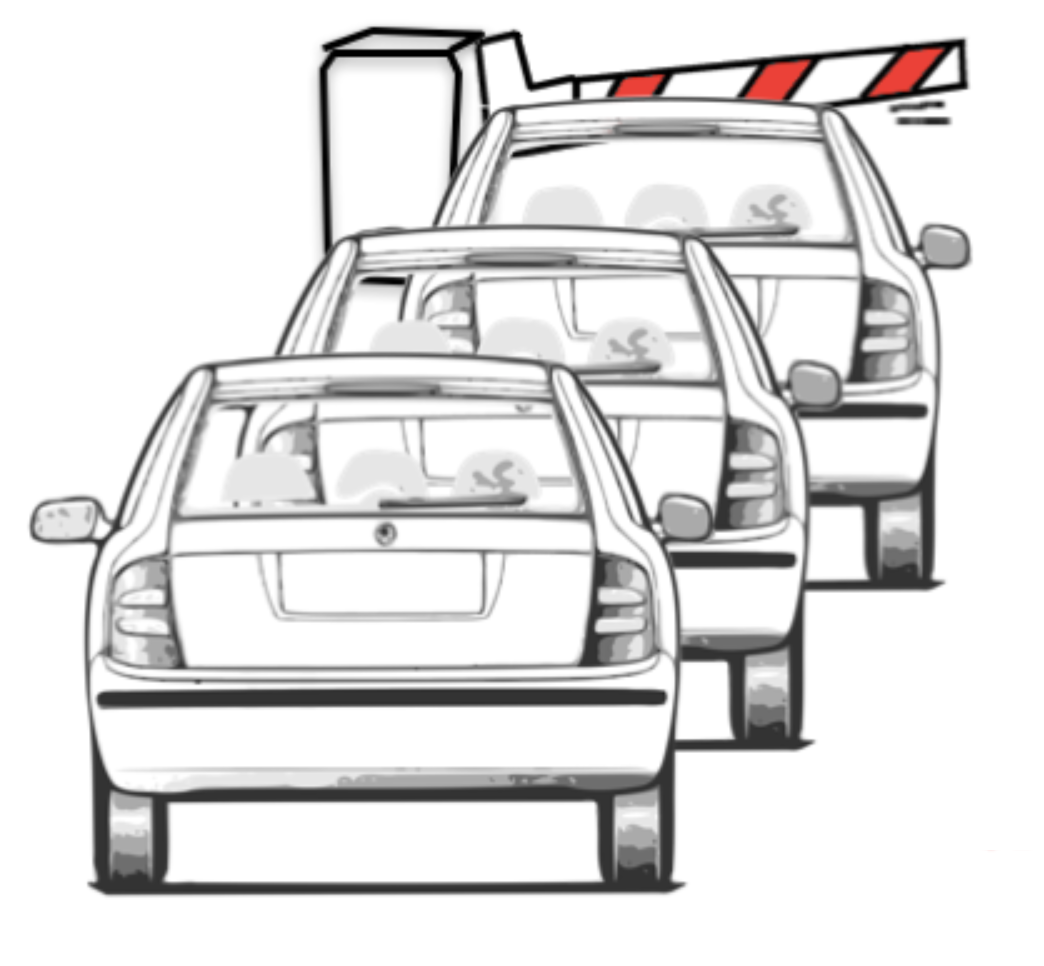
\includegraphics[width=0.7\textwidth]{latch_cars.png}
\end{center}
\end{frame}

\begin{frame}{Timing is Key, Or Else\ldots}
    
\begin{center}
    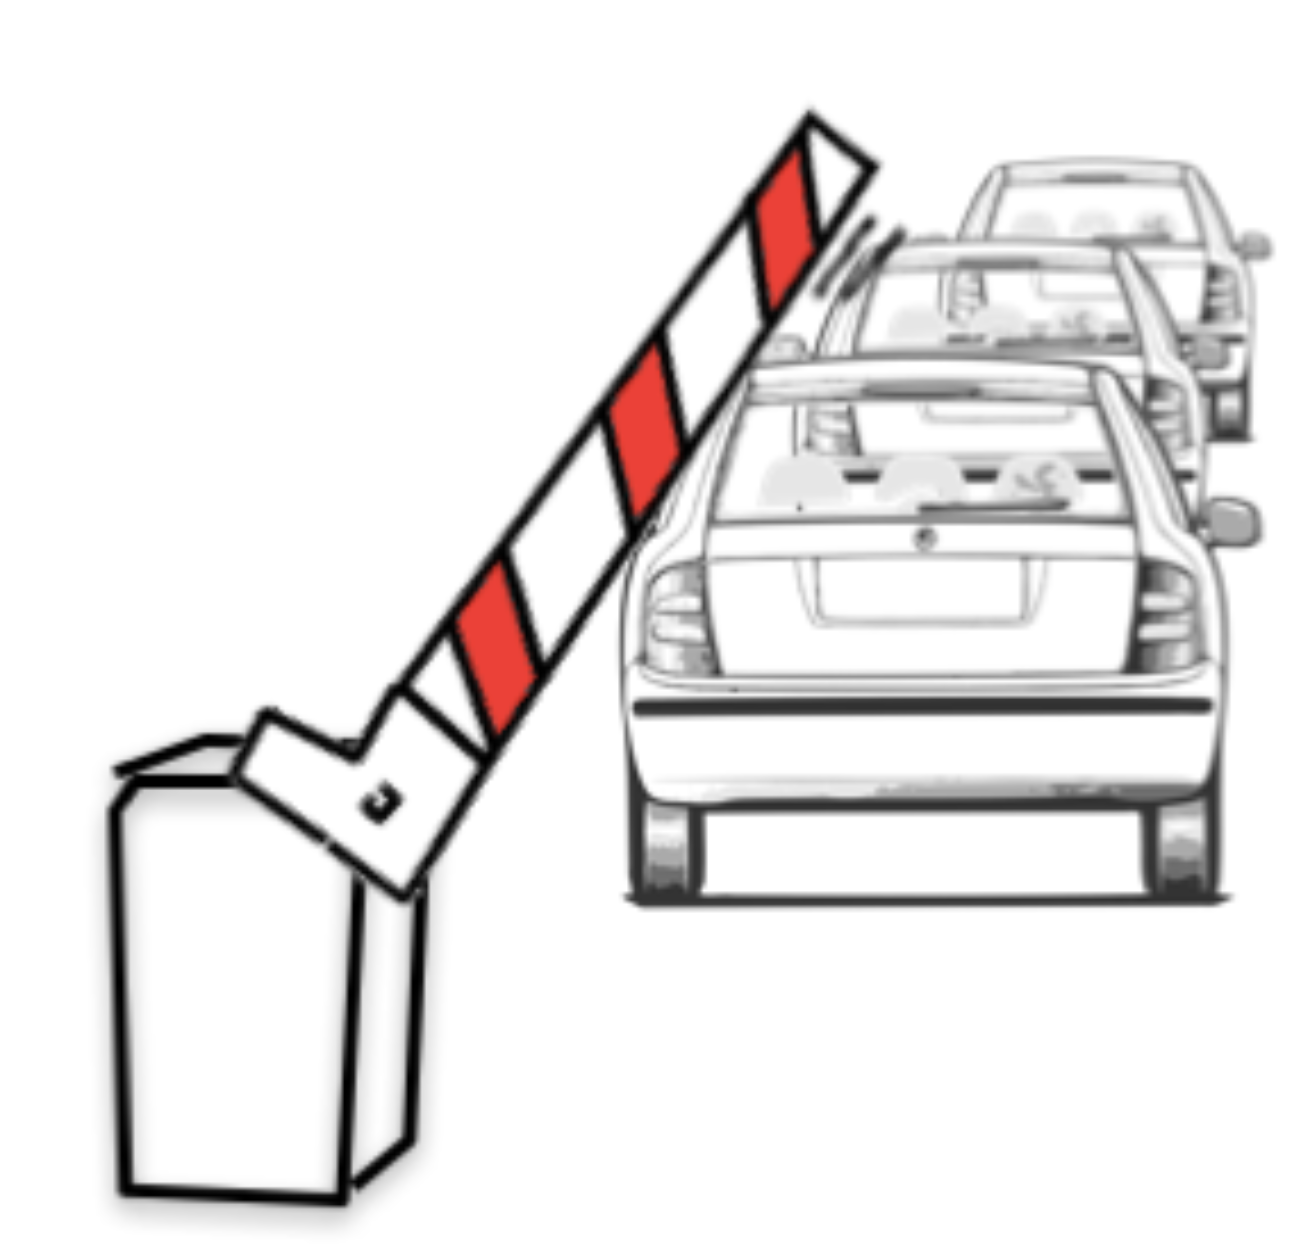
\includegraphics[width=0.7\textwidth]{latch_cars_issue.png}
\end{center}
\end{frame}



\begin{frame}{}
      \begin{center}
    {\color{sigma@mainblue} \bfseries Any ideas?}
  \end{center}
\end{frame}

\begin{frame}{Use Two Barriers!}
 \begin{columns}
\begin{column}{0.5\textwidth}
\begin{center}
    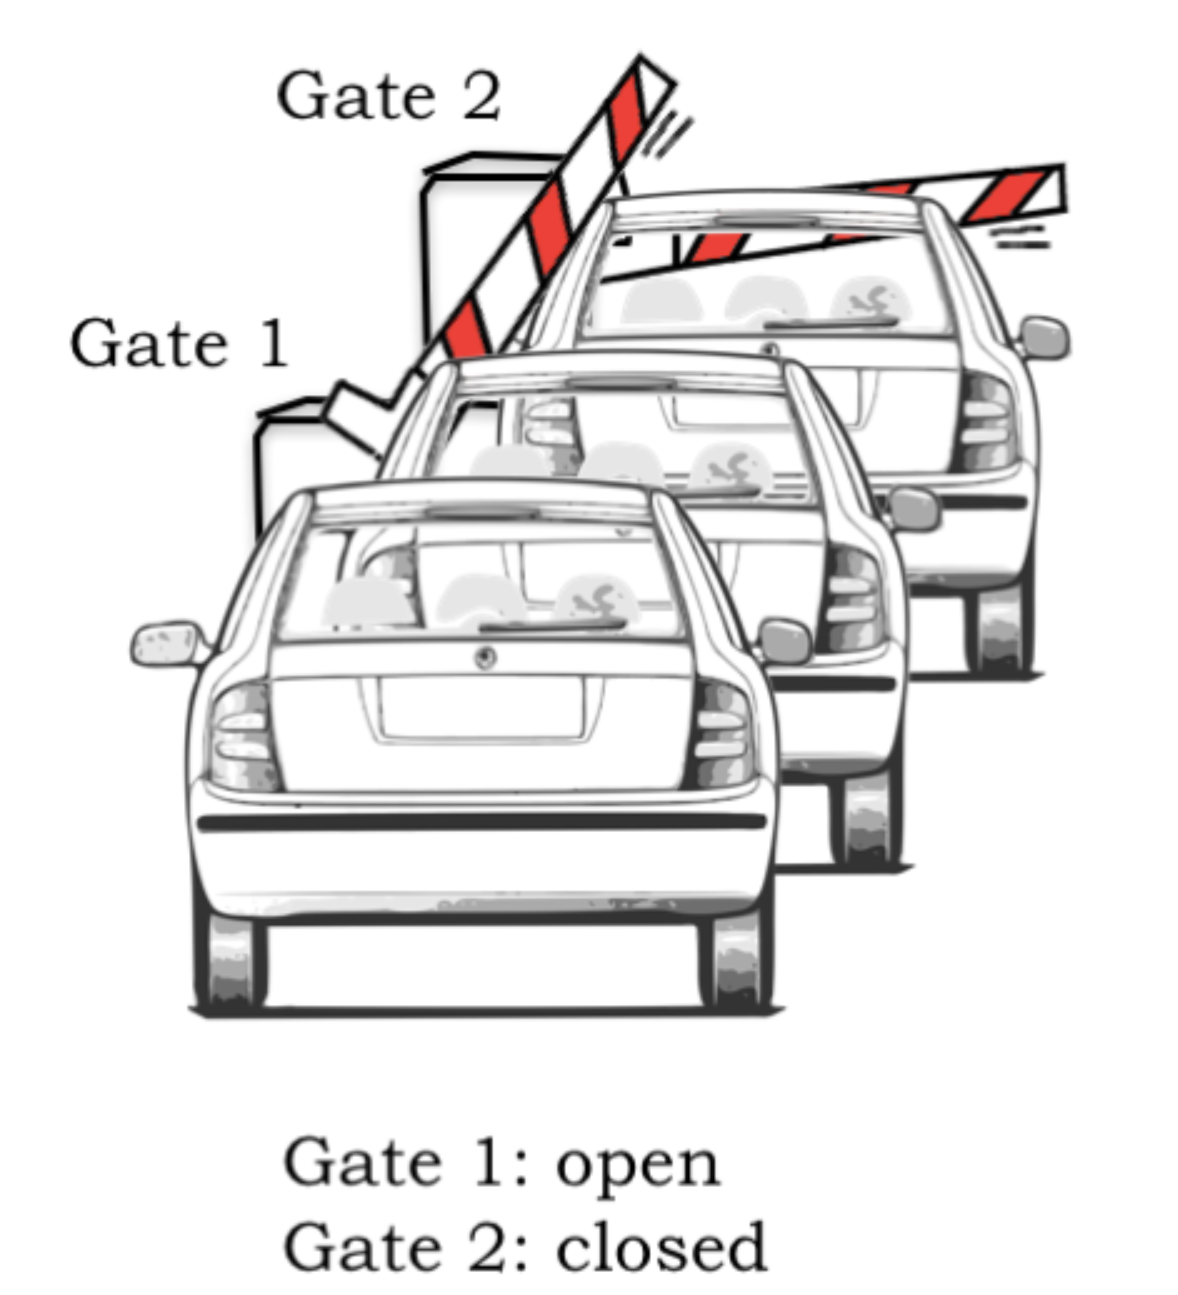
\includegraphics[width=\textwidth]{ff_cars_1.png}
\end{center}
\end{column} 
\begin{column}{0.5\textwidth}
\begin{center}
    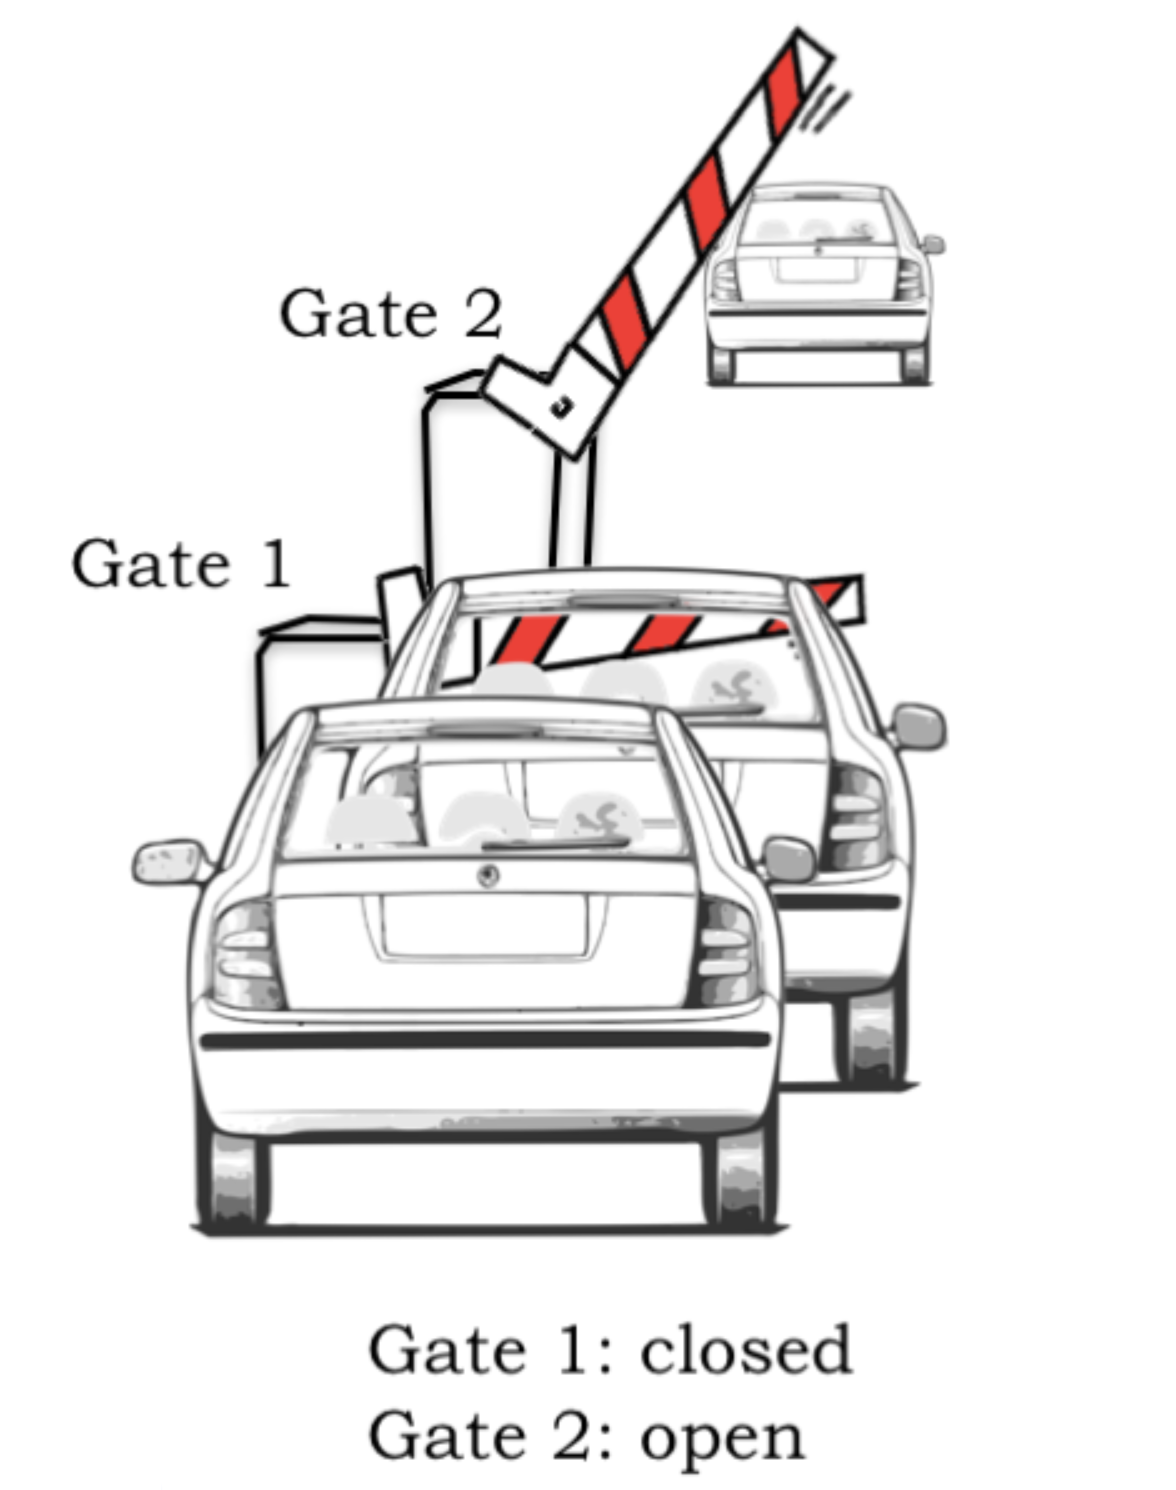
\includegraphics[width=0.9\textwidth]{ff_cars_2.png}
\end{center}
\end{column} 
 \end{columns}   
\end{frame}

\begin{frame}{How Does This Help?}
    
    \begin{itemize}
        \item Timing is now easy --- we just need to push one switch to swap the states of the barriers.\pause
        \item Actually making two barriers in hardware isn't very tricky\ldots
    \end{itemize}
\end{frame}

\begin{frame}{D Flip Flop/ D Register...Finally a Nice Storage Element!}
    \begin{center}
        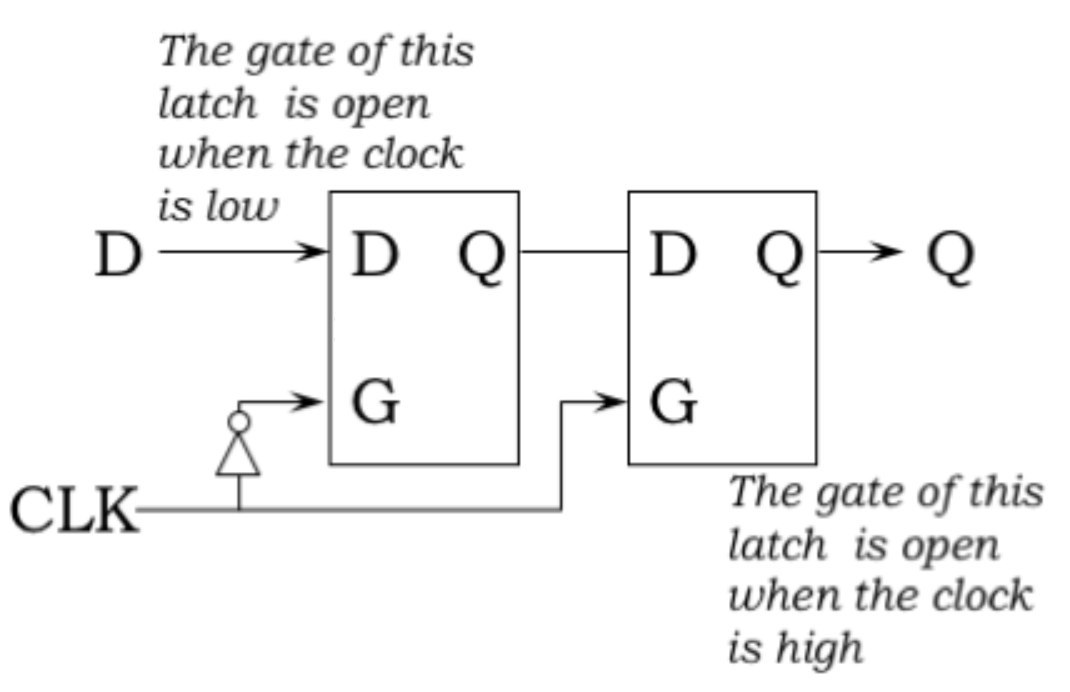
\includegraphics[width=0.8\textwidth]{ff_latch.png}
    \end{center}
\end{frame}

\begin{frame}{Who Flips the Switch?}
   What we really need is a \textbf{low to high transition}, to load data correctly into our flip flop.\\ \pause
   
   We use an alternating signal, called a clock, to give us these transitions at regular intervals.\pause
   
   \begin{center}
       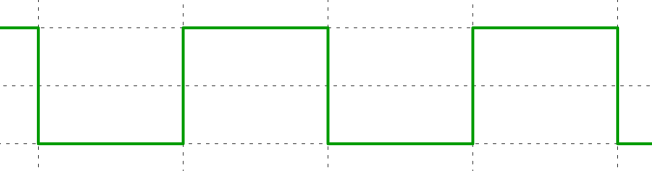
\includegraphics[width=\textwidth]{Waveforms.svg.png}
   \end{center}
    
\end{frame}

\begin{frame}{Synchronous Digital Logic}
    A synchronous digital circuit is made up of flip flops/latches and combinational logic, all run by a single clock.\\
    
\end{frame}



\begin{frame}{}
      \begin{center}
    {\color{sigma@mainblue} \bfseries\LARGE Questions?}
  \end{center}
\end{frame}

\begin{frame}{Questions!}
You're given a D flip flop, a NOT gate, and a clock signal. Make a circuit that, on every 0 to 1 transition of the clock, inverts the value stored in the flip flop. You may assume the flip flop is initialized with a valid value.\\

\textbf{Hint}: Think about when the flip flop loads data, and what data it should load.
\end{frame}

\begin{frame}{Solution}
    \begin{center}
        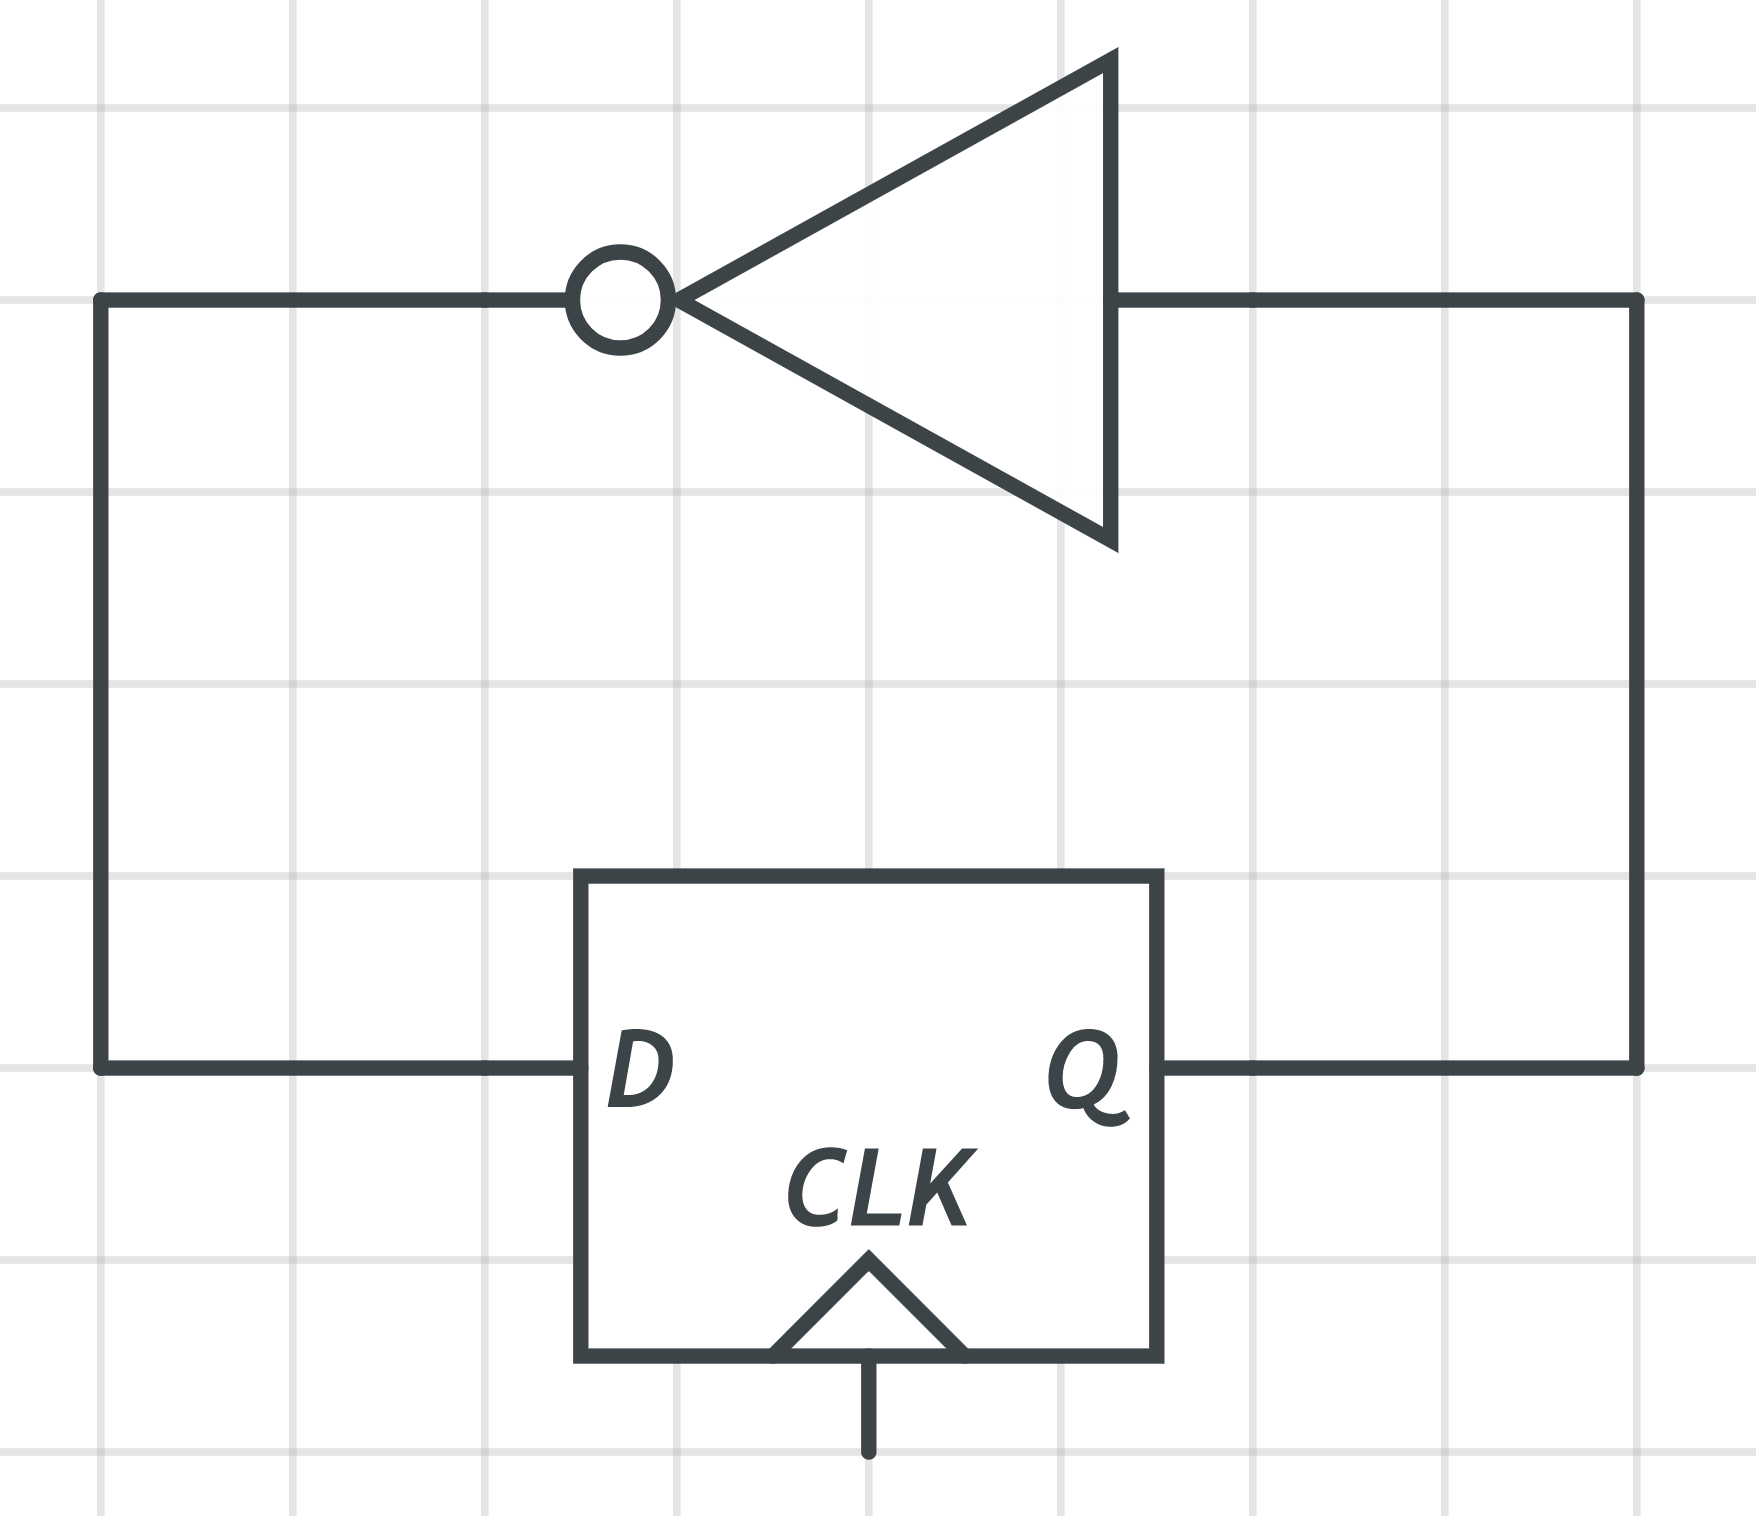
\includegraphics[width=0.6\textwidth]{dff_not.png}
    \end{center}
\end{frame}

\begin{frame}{We Can Now Build FSMs!}
    Recall that a DFA is simply something like:
    \begin{center}
        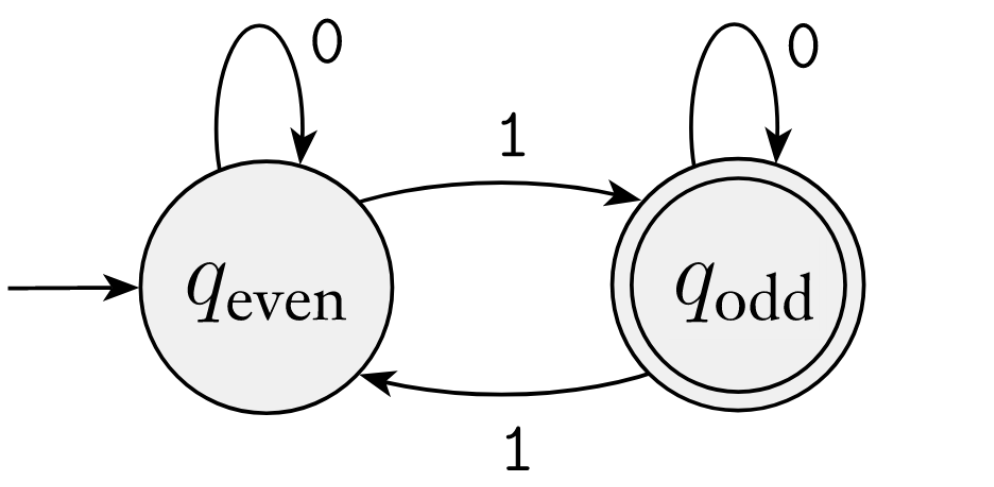
\includegraphics[width=0.8\textwidth]{oddDFA.png}
    \end{center}
    \pause
    
    Let's build something similar\footnote{Formally, a finite state transducer.} using our synchronous logic.
    
\end{frame}

\begin{frame}{What is an FSM, \emph{Really}}
\begin{columns}


\begin{column}{0.5\textwidth}
    \begin{center}
        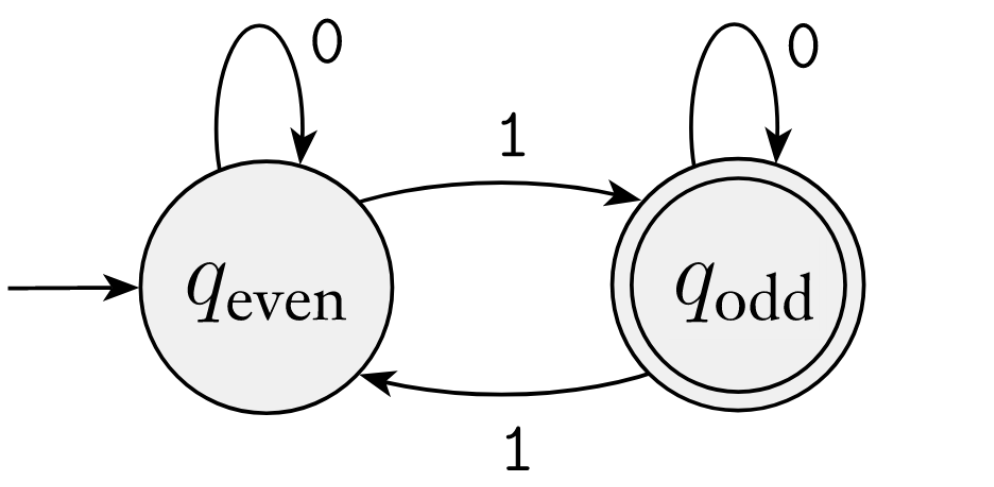
\includegraphics[width=0.8\textwidth]{oddDFA.png}
    \end{center}
\end{column}\pause
\begin{column}{0.5\textwidth}
    \begin{itemize}
        \item An input alphabet\pause :~$\{0,\,1\}$\pause
        \item A bunch of states\pause :~$\{q_{even},\,q_{odd} \}$\pause
        \item An initial state\pause :~$q_{even}$\pause
        \item A state transition function\pause :
        
\begin{center}
\begin{tabular}{cc|c}
\toprule
State & Input & Next State\\
\midrule
\(q_{\mathrm{even}}\) & 0 & \(q_{\mathrm{even}}\)\\
\(q_{\mathrm{even}}\) & 1 & \(q_{\mathrm{odd }}\)\\
\(q_{\mathrm{odd }}\) & 0 & \(q_{\mathrm{odd }}\)\\
\(q_{\mathrm{odd }}\) & 1 & \(q_{\mathrm{even}}\)\\
\bottomrule
\end{tabular}
\end{center}

    \end{itemize}
\end{column}
\end{columns}

\end{frame}


\begin{frame}{Now, Let's Make it in Hardware}

\begin{columns}

\begin{column}{0.5\textwidth}
    \begin{itemize}
        \item An input alphabet:~$\{0,\,1\}$
        \item A bunch of states:~$\{q_{even},\,q_{odd} \}$
        \item An initial state:~$q_{even}$
        \item A state transition function:
        
\begin{center}
\begin{tabular}{cc|c}
\toprule
State & Input & Next State\\
\midrule
\(q_{\mathrm{even}}\) & 0 & \(q_{\mathrm{even}}\)\\
\(q_{\mathrm{even}}\) & 1 & \(q_{\mathrm{odd }}\)\\
\(q_{\mathrm{odd }}\) & 0 & \(q_{\mathrm{odd }}\)\\
\(q_{\mathrm{odd }}\) & 1 & \(q_{\mathrm{even}}\)\\
\bottomrule
\end{tabular}
\end{center}

    \end{itemize}
\end{column}\pause

\begin{column}{0.5\textwidth}
    \begin{itemize}
        \item An input alphabet:~$\{0,\,1\}$\pause
        \item A bunch of states\pause :~use a flip flop, $(q_{\mathrm{even}}, q_{\mathrm{odd}}) = (0,\, 1)$. \pause
        \item An initial state\pause :~initialize the flip flop to 0.\pause
        \item A state transition function\pause:
        \begin{center}
\begin{tabular}{cc|c}
\toprule
State & Input & Next State\\
\midrule
0 & 0 & 0\\
0 & 1 & 1\\
1 & 0 & 1\\
1 & 1 & 0\\
\bottomrule
\end{tabular}
\end{center}

        
    \end{itemize}
\end{column}
    \end{columns}
\end{frame}

\begin{frame}{Our Final Hardware FSM Is}
    \begin{center}
        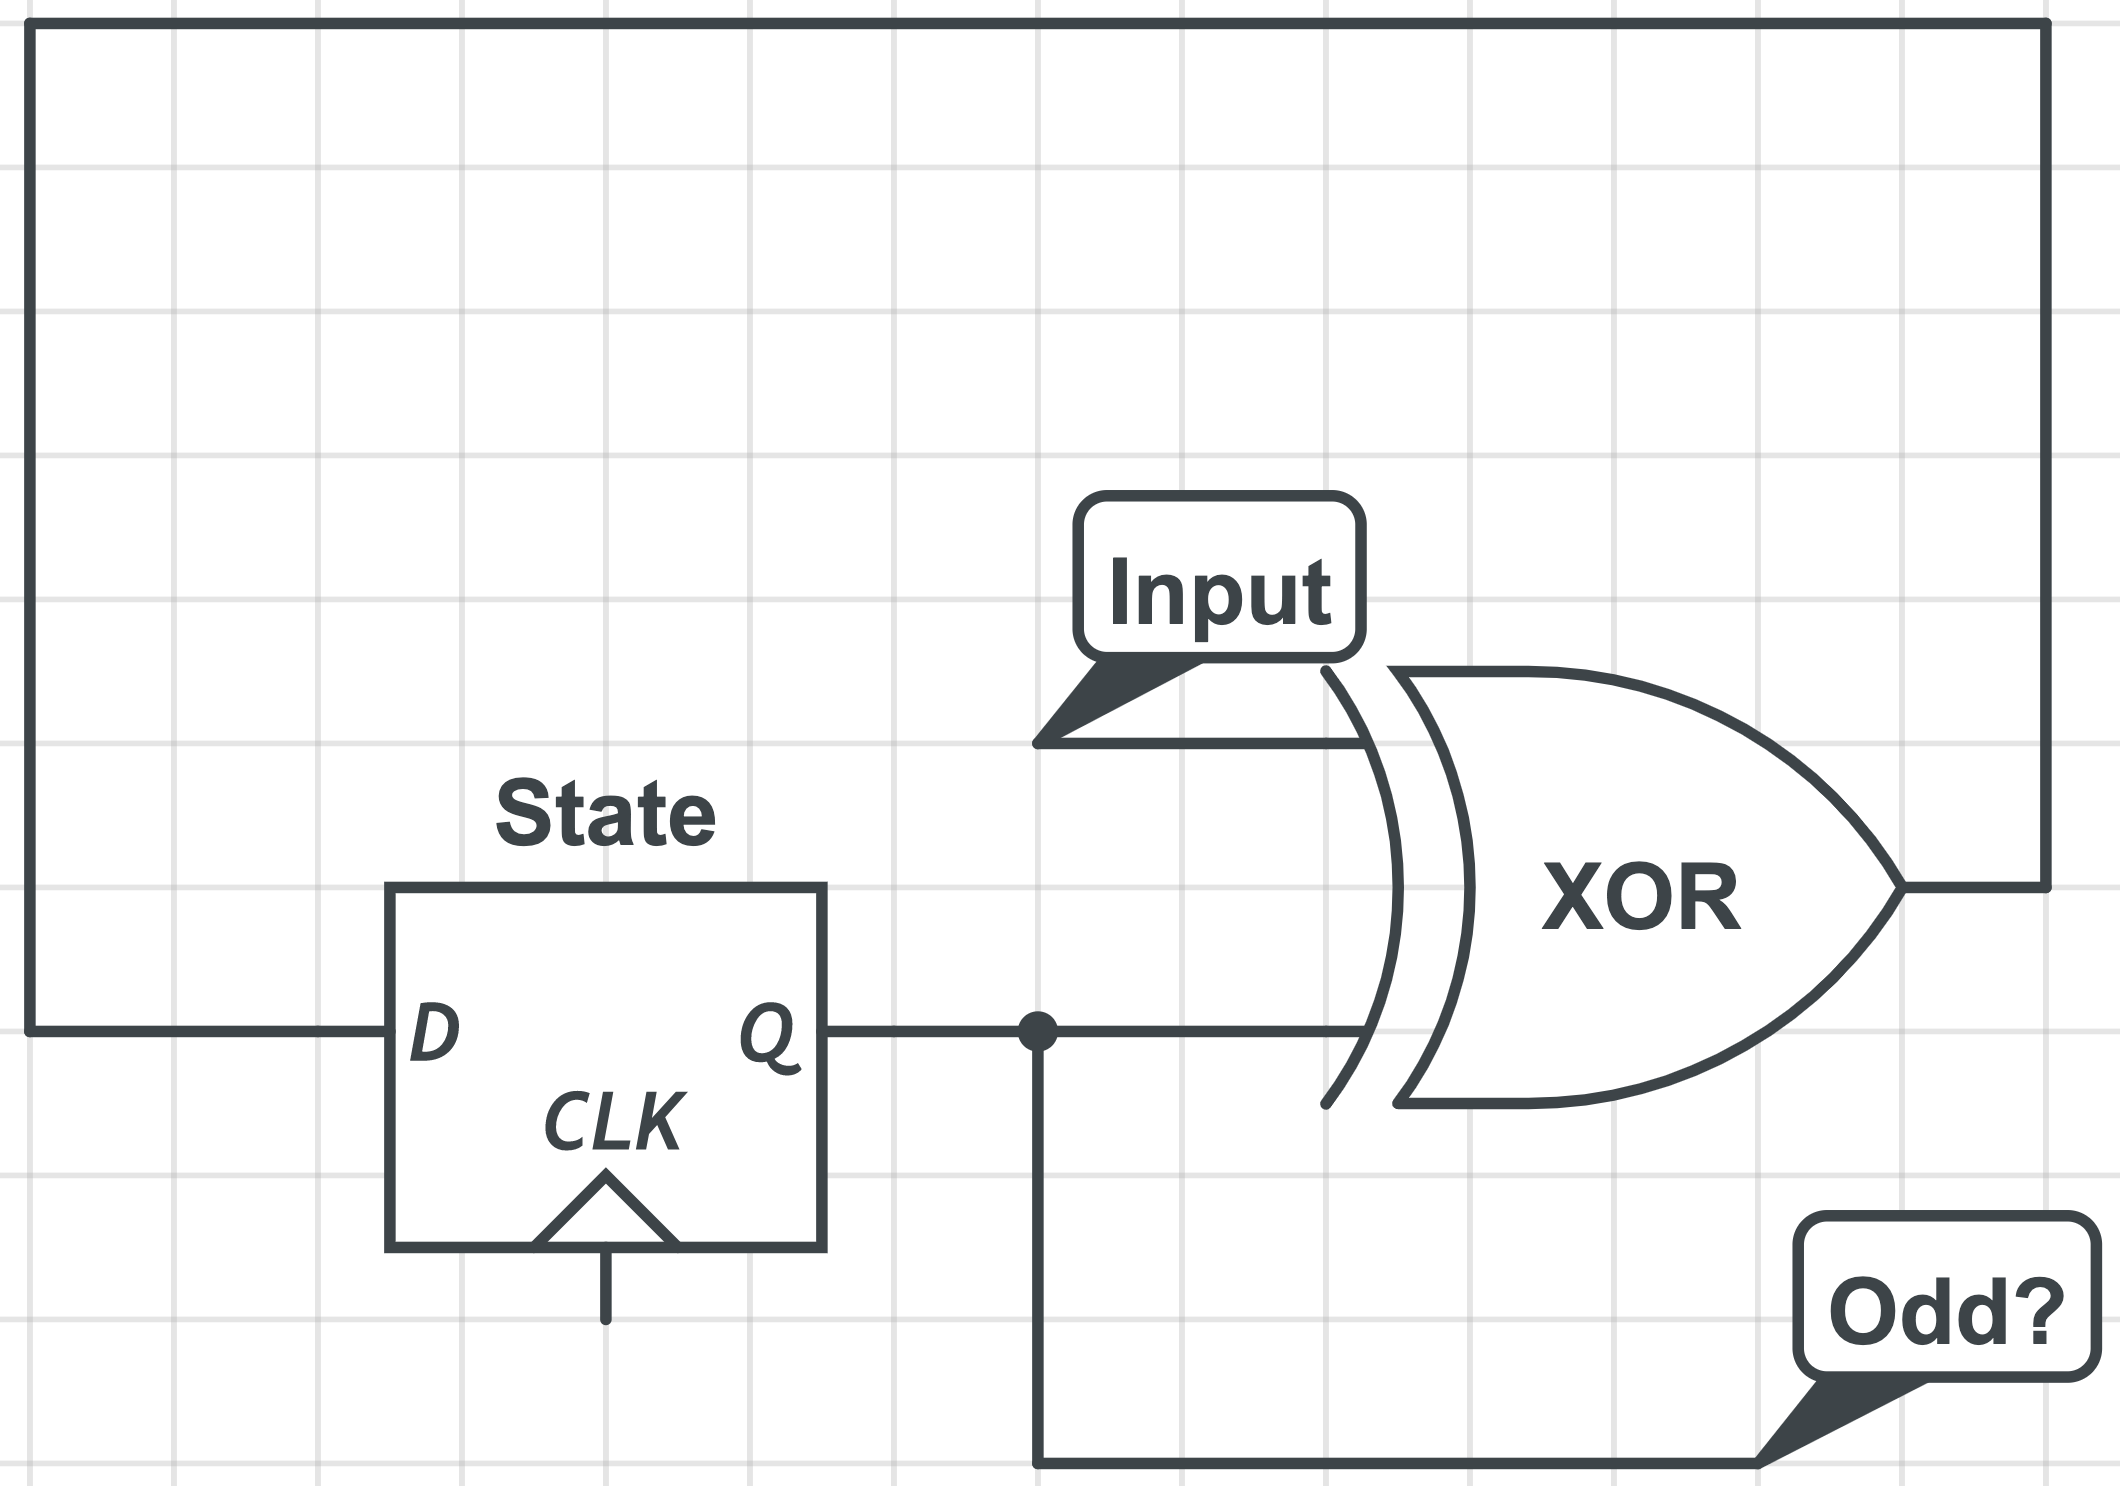
\includegraphics[width=0.75\textwidth]{Screen Shot 2022-09-25 at 02.09.53.png}
    \end{center}
\end{frame}

\begin{frame}{Hardware FSMs Also Have Outputs}
% In our FSM, we use the state as an output to tell us whether we've read an odd number of 1's. In general, our FSMs have, in addition to the usual stuff,\ldots
    \begin{itemize}
        \item An output alphabet
        \item An output function that maps states to outputs
    \end{itemize}
    
\end{frame}

\begin{frame}{Generalized (Moore) FSM Architecture}
    \begin{center}
        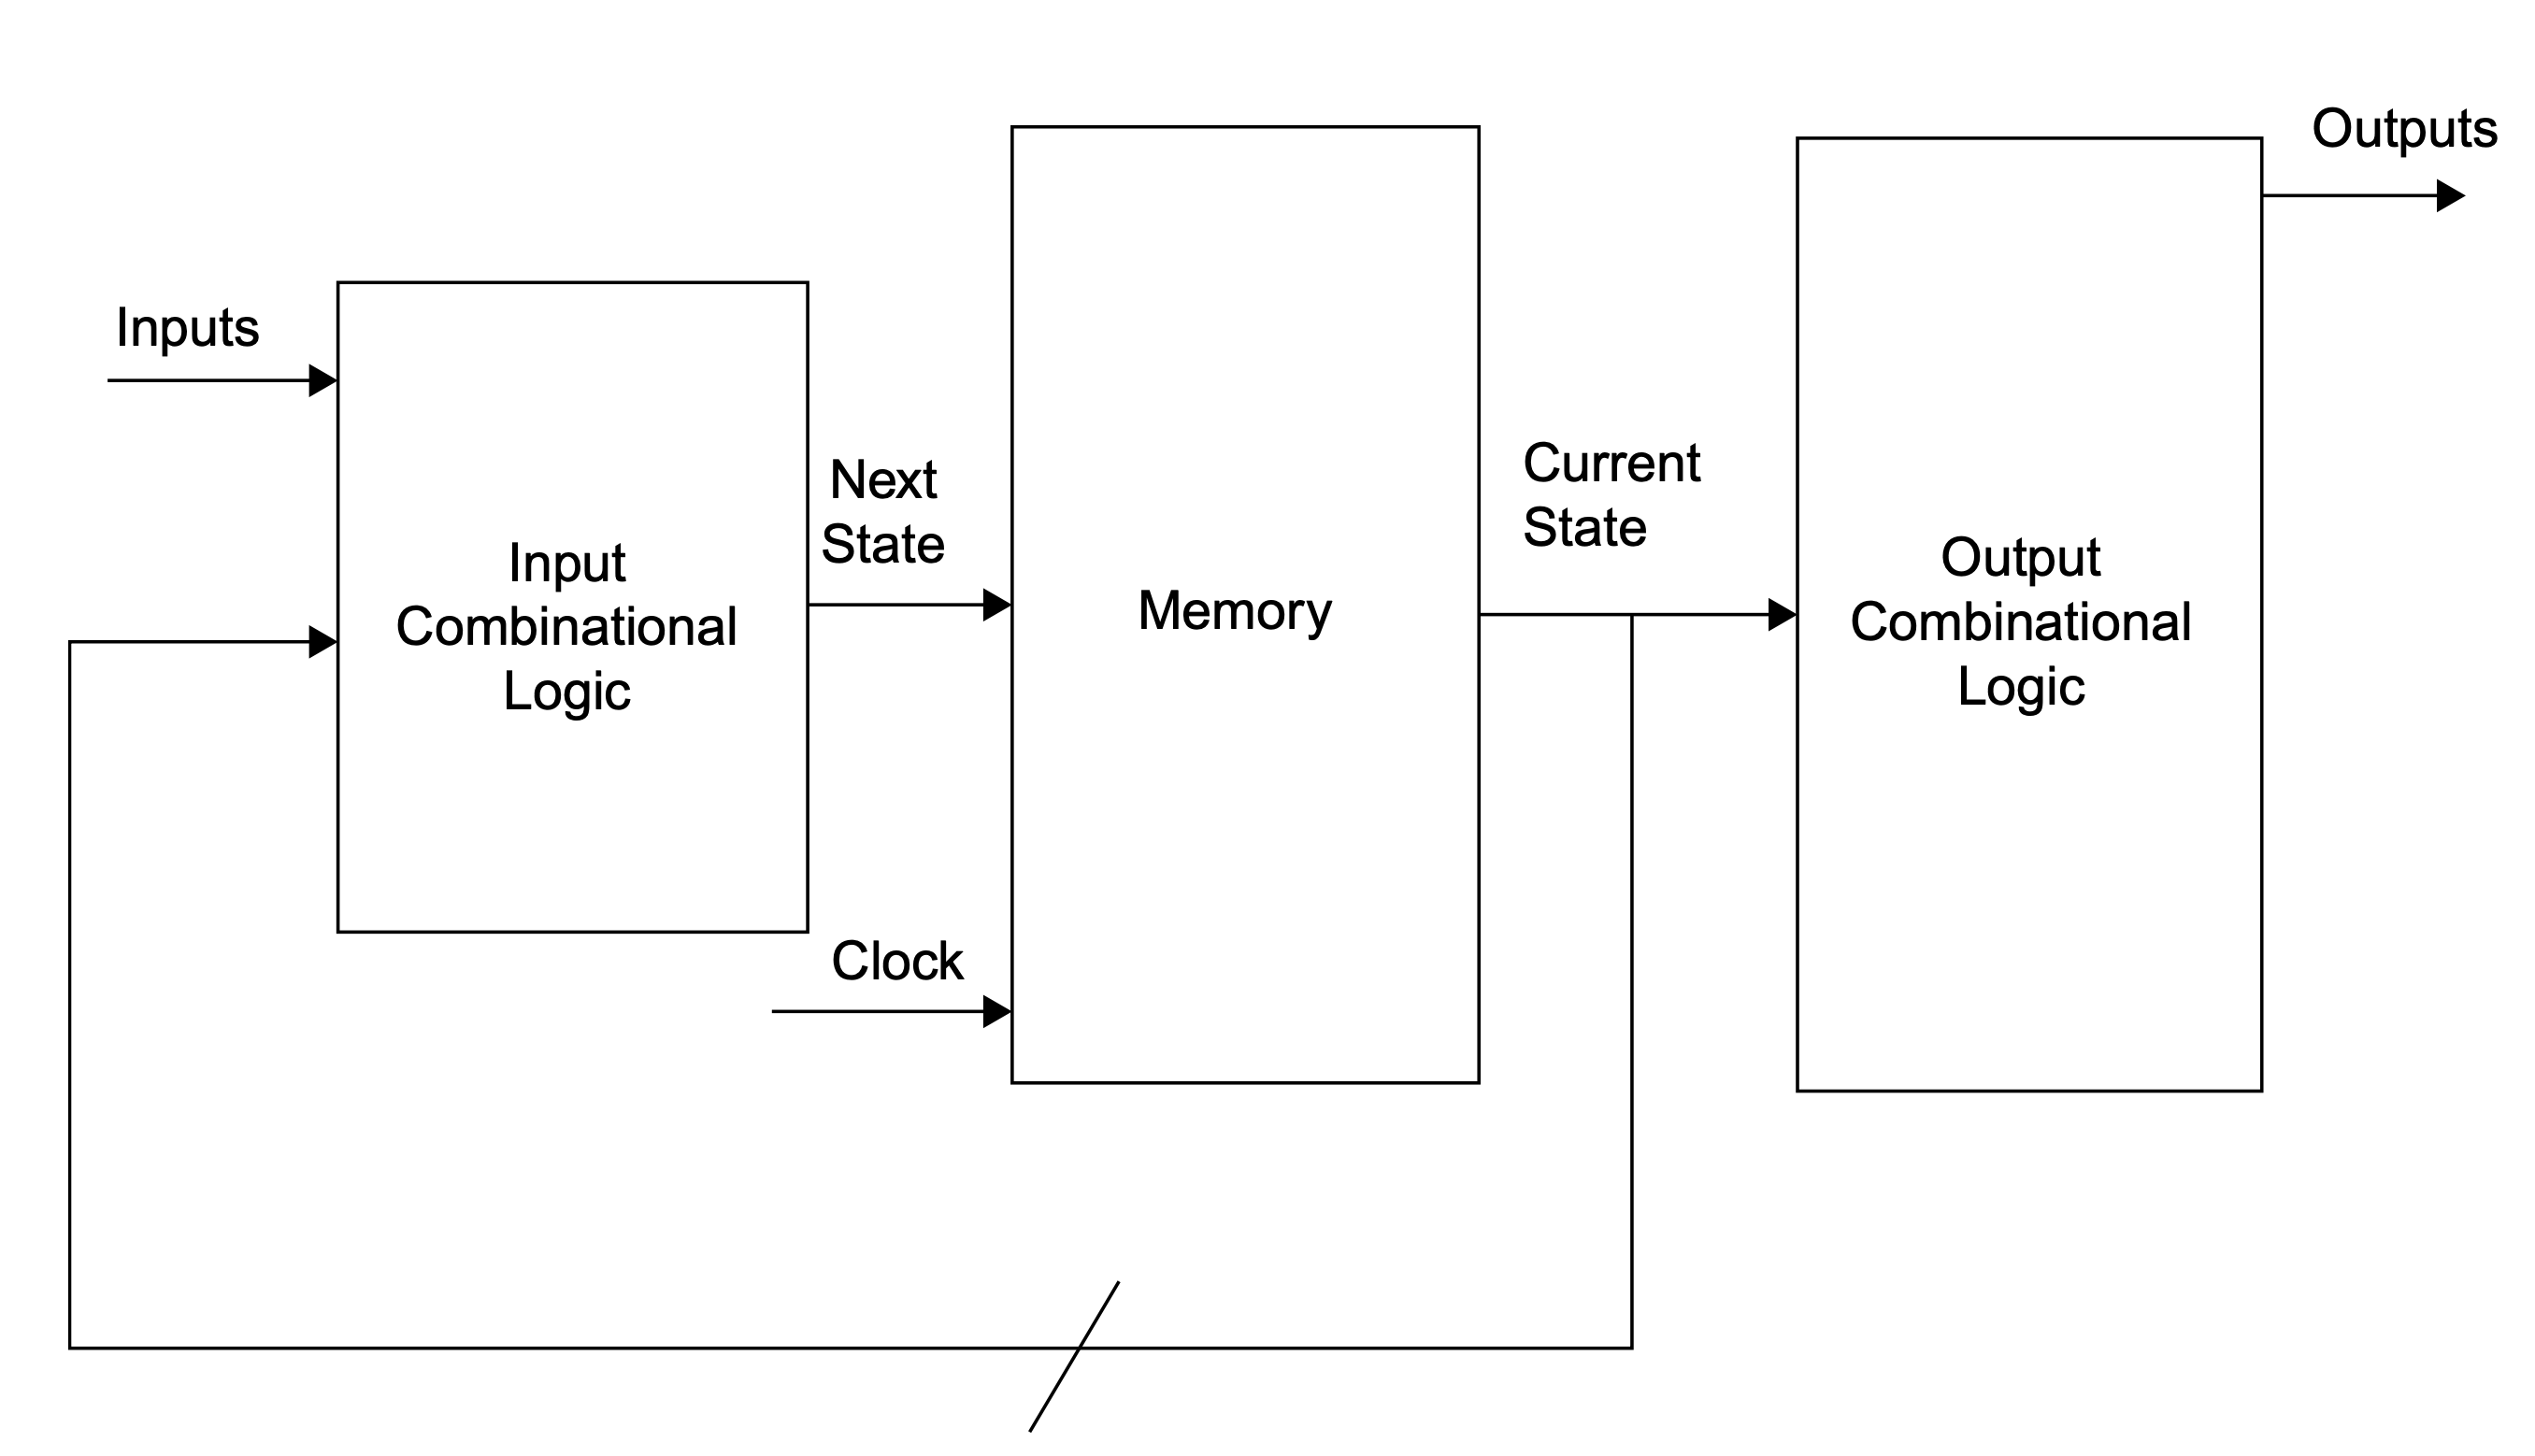
\includegraphics[width=\textwidth]{Screen Shot 2022-09-25 at 02.25.15.png}
    \end{center}
\end{frame}


\begin{frame}{}
      \begin{center}
    {\color{sigma@mainblue} \bfseries\LARGE Questions?}
  \end{center}
\end{frame}

\begin{frame}{Questions!}
    Design in hardware an FSM that detects non-overlapping sequences of the string 101. (Your input alphabet is $\{0,\,1\}$.)
\end{frame}

\section{Building a Computer}
\frame{\sectionpage}


\begin{frame}{What is a Computer?}
    \pause
    According to Wikipedia\ldots
    
\begin{quote}    
   A computer is a digital electronic machine that can be programmed to carry out sequences of arithmetic or logical operations (computation) automatically. 
   \end{quote}
   
   Surprisingly accurate description --- of a CPU.
\end{frame}

\begin{frame}{Von Neumann Architecture}
    
    \begin{center}
        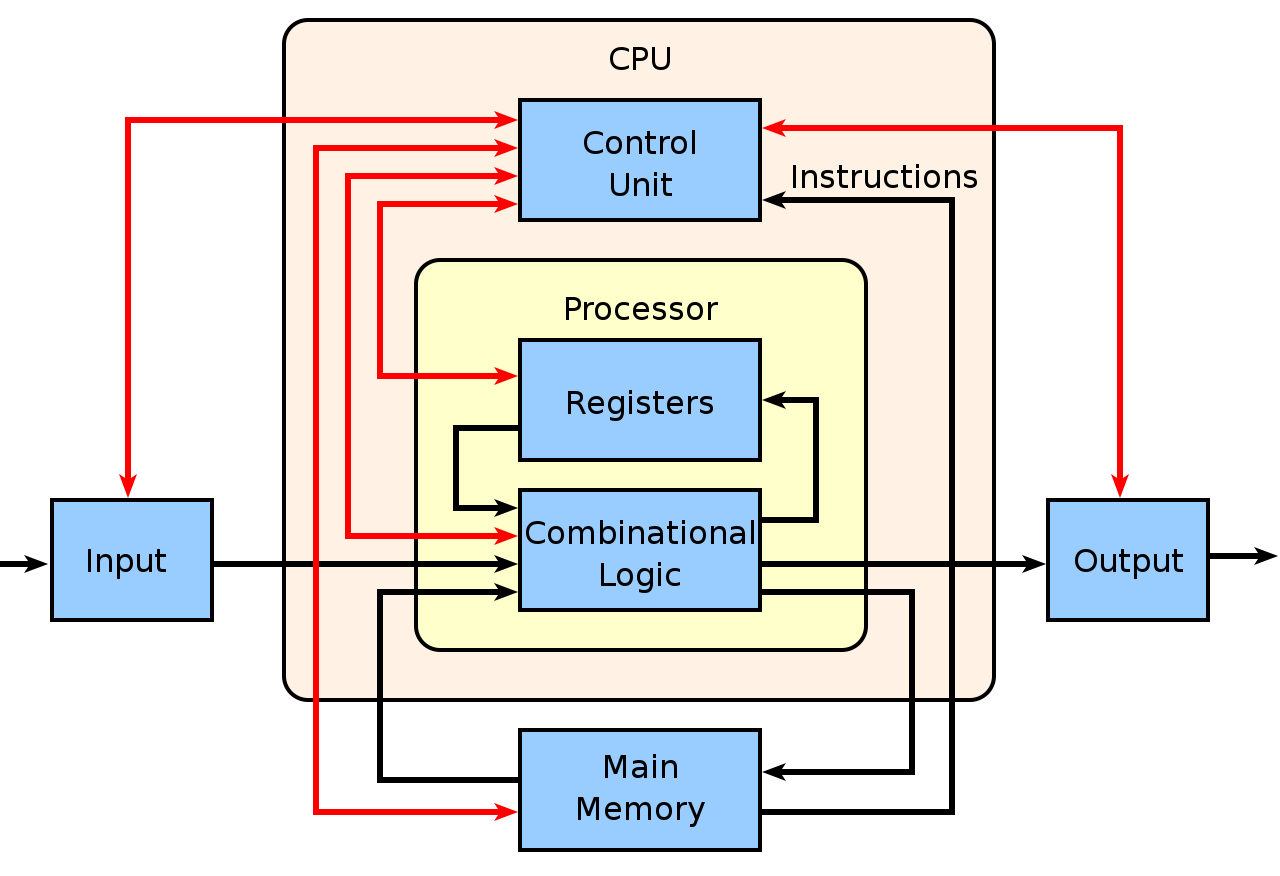
\includegraphics[width=0.7\textwidth]{1280px-ABasicComputer.png}
    \end{center}
\end{frame}

\begin{frame}{A CPU Has}
\pause
    \begin{itemize}
        \item \textbf{Memory}: We'll assume it's random access. The CPU can read/write values from here at will.\pause
        \item \textbf{Registers}: a bunch of flip flops where it stores values that it's currently operating on.\pause
        \item \textbf{Combinational logic} to ``compute'' things: adders, logical units, etc. whose inputs and outputs are the registers.\pause
        \item \textbf{Instructions}: Stored in the memory, (logically) executed one after another.\pause
        \item \textbf{Control Unit}: Orchestrates the whole thing.
    \end{itemize}
\end{frame}

\begin{frame}{The Control Unit Is}
    A giant FSM that does the following things:\pause
    \begin{itemize}
        \item \textbf{Fetch}: Gets an ``instruction'' from memory.\pause
        \item \textbf{Decode}: Figures out what to do according to the instruction.\pause
        \item \textbf{Execute}: Actually do the instruction. Once it's done, go decode the next instruction in memory --- increment the program counter.
    \end{itemize}
    
\end{frame}


\begin{frame}{Instructions}
    What can the CPU do?
    \begin{itemize}
        \item \texttt{ADD}: Takes two registers, adds them, puts the sum in a register. Set condition codes.\pause
        \item \texttt{AND}: Takes two registers, ANDs them, puts the result in a register. Set condition codes.\pause
        \item \texttt{NOT}: Takes a register, NOTs it, puts the result in a register. Set condition codes.\pause
        \item \texttt{BR}: Depending on ``condition codes'', move the program counter to the location specified.\pause
        \item \texttt{JMP}: Move the program counter to the address specified.\pause
        \item \texttt{LDR}: Load the contents of a memory address into a register.\pause
        \item \texttt{STR}: Store the contents of a register into a memory address.
    \end{itemize}
\end{frame}

\begin{frame}{}
    \begin{center}
        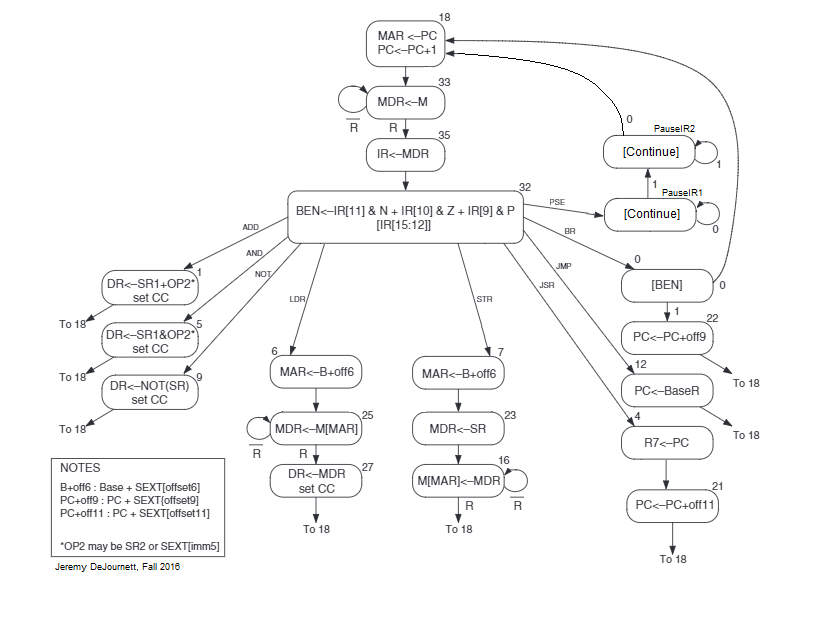
\includegraphics[width=\textwidth]{statediagram.png}
    \end{center} 
\end{frame}

\begin{frame}{}
    \begin{center}
        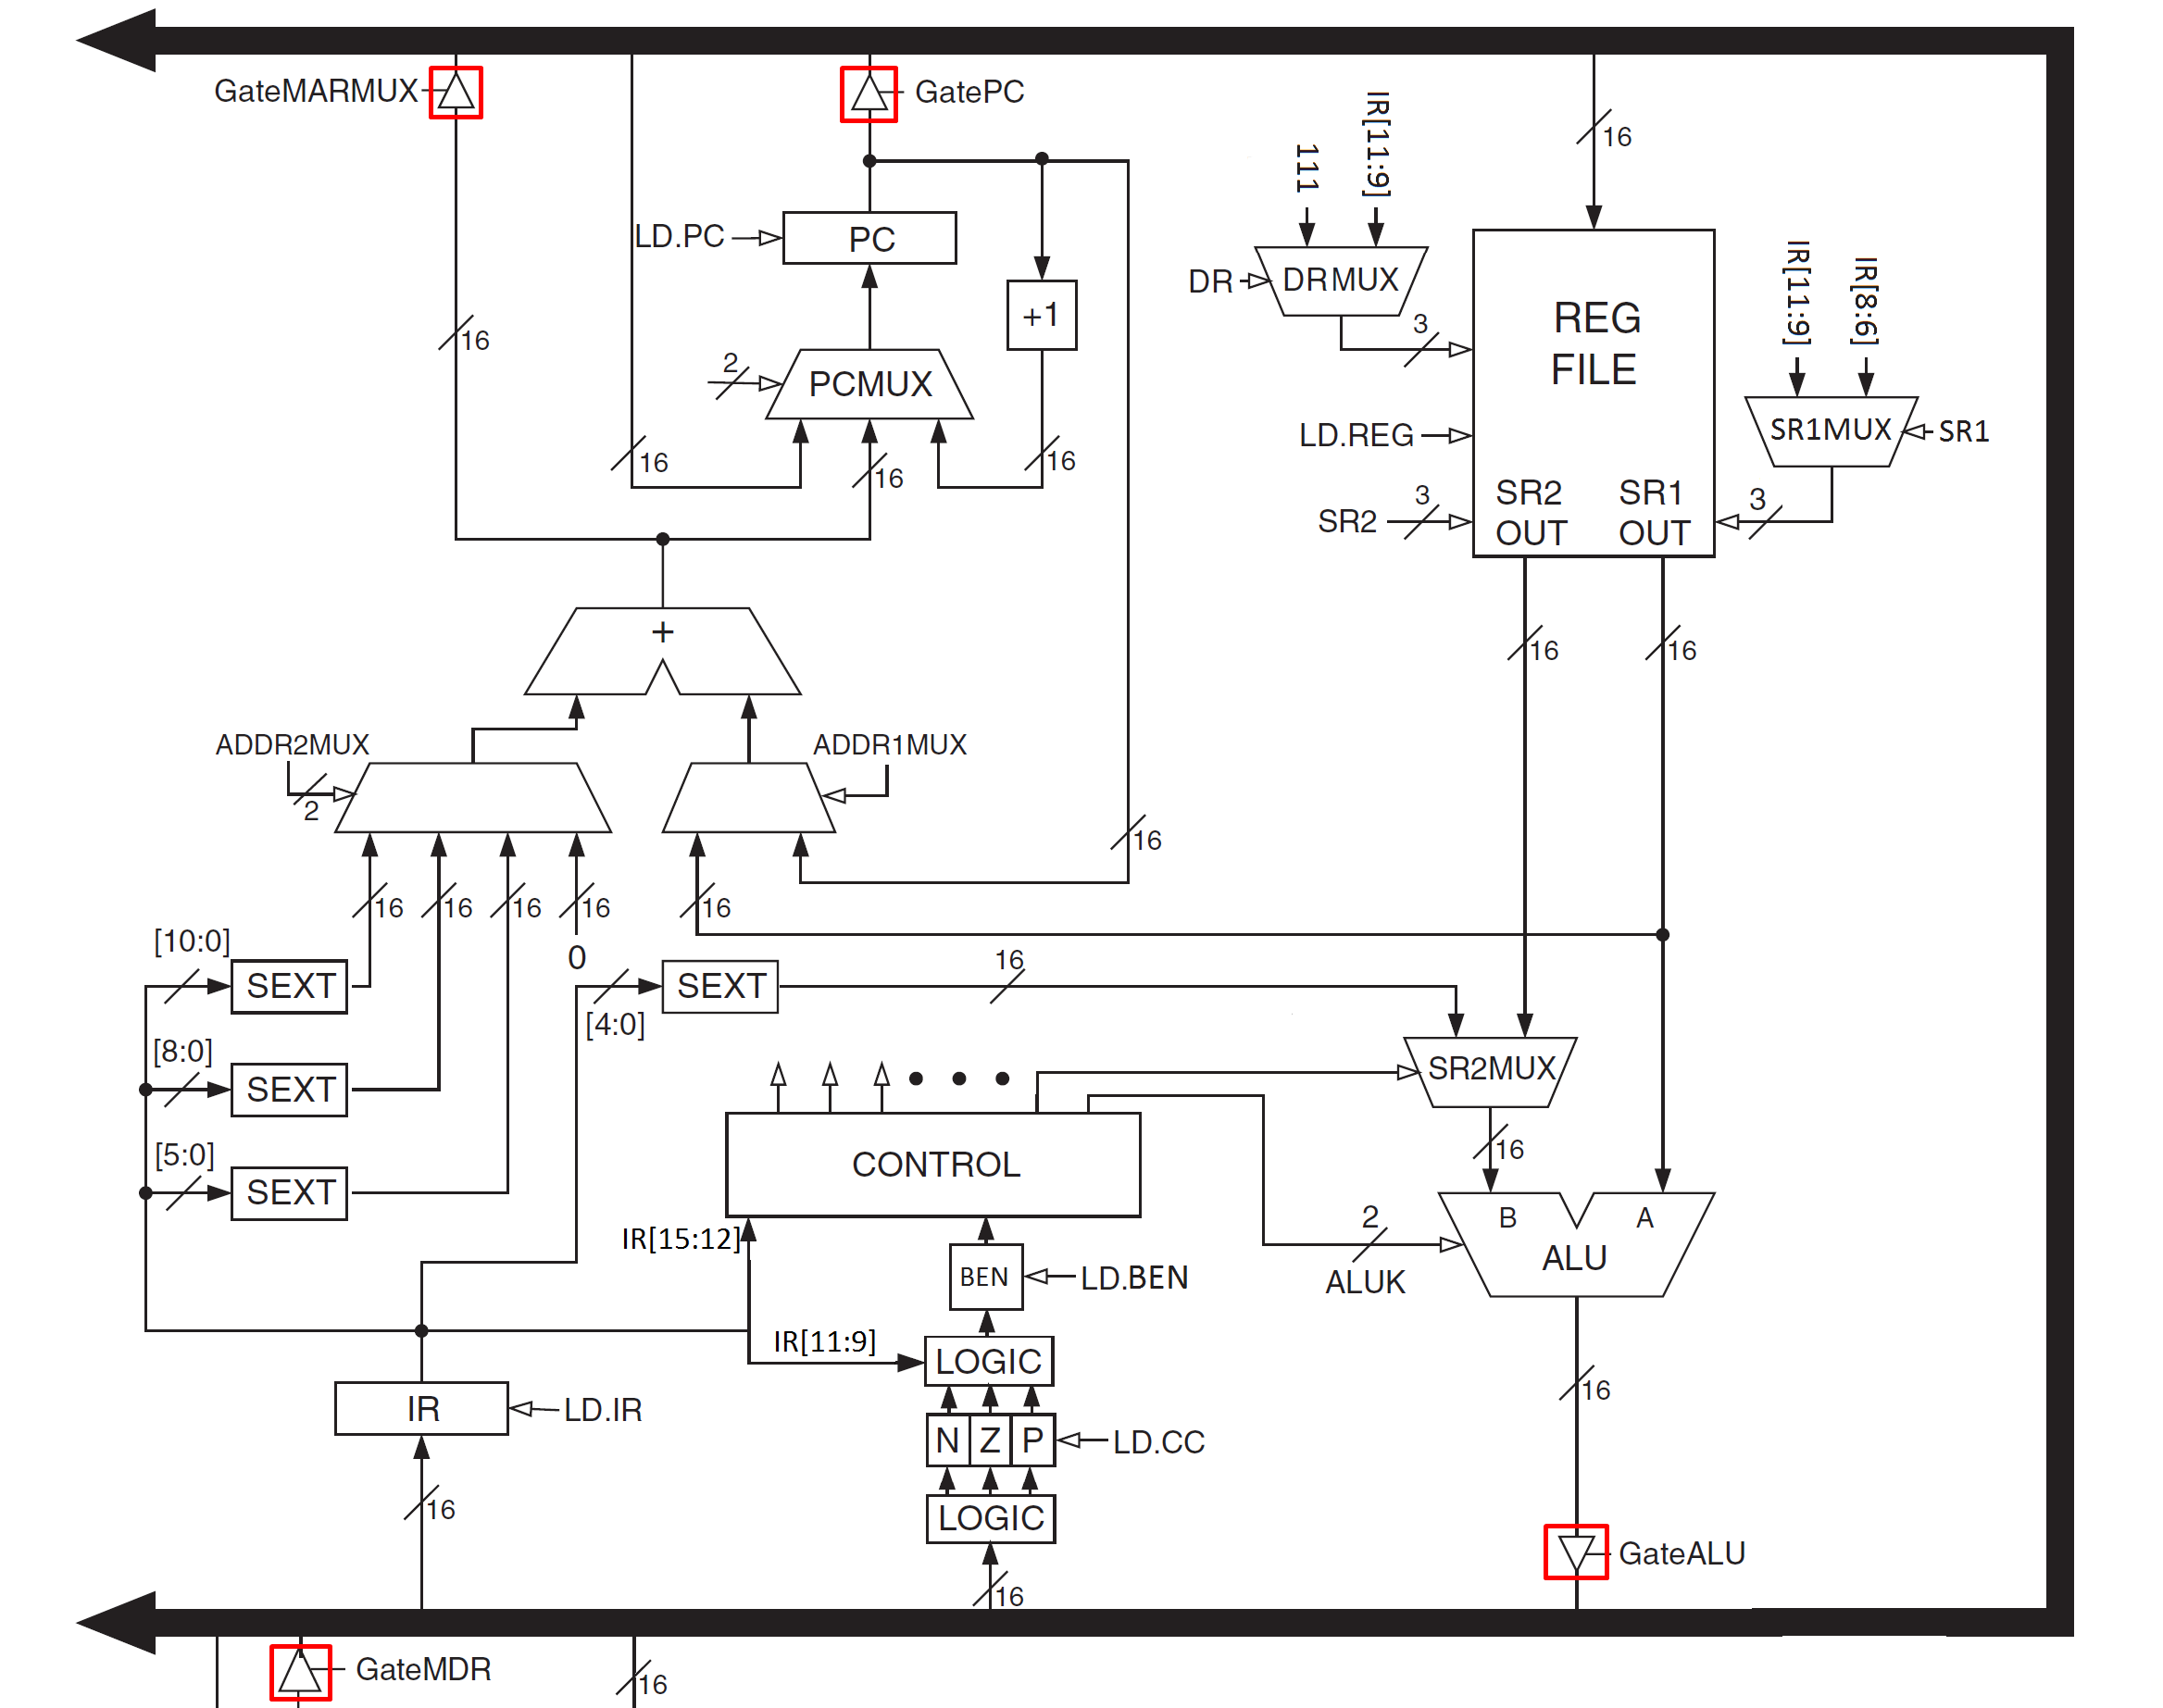
\includegraphics[width=0.85\textwidth]{SLC3_updated.png}
    \end{center}
\end{frame}

\font\eightss=cmssq8
\font\eightssi=cmssqi8
\newcommand\quoteAuthorDate[3]{\begingroup
  \baselineskip 10pt
  \parfillskip 0pt
  \interlinepenalty 10000 % not needed in example
  \leftskip 0pt plus 40pc minus \parindent
  \let\rm=\eightss
  \let\sl=\eightssi
  \everypar{\sl}#1\par
  \nobreak\smallskip
  \noindent\rm--- #2\unskip\enspace(#3)\par
  \endgroup}


\begin{frame}{}
      \begin{center}
    {\color{sigma@mainblue} \bfseries\LARGE Questions?}
  \end{center}
\end{frame}

\begin{frame}{42}
    \centering
    \quoteAuthorDate{
The computer looked normal size for a black space-borne 
computer satellite --- about a thousand miles across.
    }{DOUGLAS ADAMS}{1979}
\end{frame}


\end{document}
